\section{Captcha Klassenreferenz}
\label{classCaptcha}\index{Captcha@{Captcha}}
Klassendiagramm für Captcha::\begin{figure}[H]
\begin{center}
\leavevmode
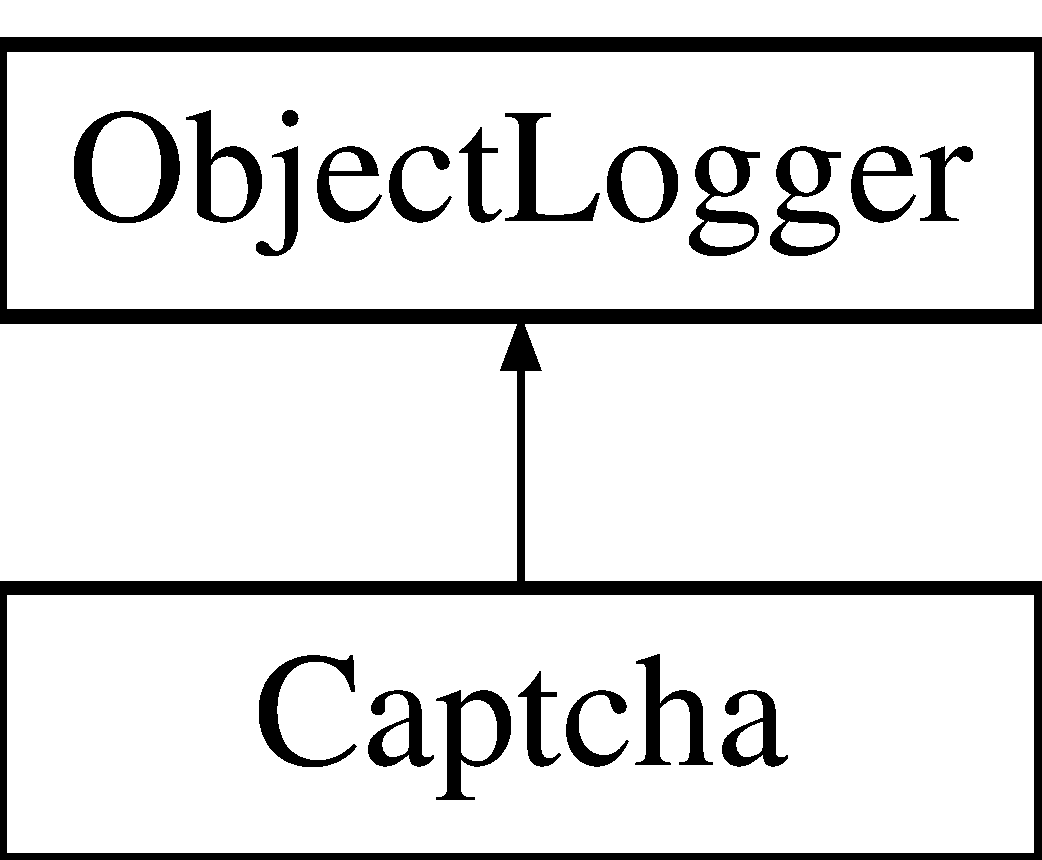
\includegraphics[height=2cm]{classCaptcha}
\end{center}
\end{figure}
\subsection*{Öffentliche Methoden}
\begin{CompactItemize}
\item 
{\bf Captcha} ()
\item 
{\bf \_\-initialize} ()
\item 
{\bf validateToken} (\$publicKey, \$privateKey)
\item 
{\bf getNewCaptchaPublicKey} ()
\end{CompactItemize}
\subsection*{Öffentliche Attribute}
\begin{CompactItemize}
\item 
{\bf \$CAPTCHA\_\-INIT}
\item 
{\bf \$\_\-captchaObj}
\end{CompactItemize}


\subsection{Ausführliche Beschreibung}


Definiert in Zeile 9 der Datei class.Captcha.php.

\subsection{Dokumentation der Elementfunktionen}
\index{Captcha@{Captcha}!Captcha@{Captcha}}
\index{Captcha@{Captcha}!Captcha@{Captcha}}
\subsubsection{\setlength{\rightskip}{0pt plus 5cm}Captcha.Captcha ()}\label{classCaptcha_2db9fbc65381d85da572c91974a44442}




Definiert in Zeile 20 der Datei class.Captcha.php.

Benutzt \_\-initialize() und ObjectLogger.setRequiredDefinitions().\index{Captcha@{Captcha}!\_\-initialize@{\_\-initialize}}
\index{\_\-initialize@{\_\-initialize}!Captcha@{Captcha}}
\subsubsection{\setlength{\rightskip}{0pt plus 5cm}Captcha.\_\-initialize ()}\label{classCaptcha_67b9ec6afec78d8f2e710256cc365dd9}




Definiert in Zeile 28 der Datei class.Captcha.php.

Benutzt ObjectLogger.\_\-validateRequiredDefinitions().

Wird benutzt von Captcha().\index{Captcha@{Captcha}!validateToken@{validateToken}}
\index{validateToken@{validateToken}!Captcha@{Captcha}}
\subsubsection{\setlength{\rightskip}{0pt plus 5cm}Captcha.validateToken (\$ {\em publicKey}, \$ {\em privateKey})}\label{classCaptcha_29247379025c1941a94caffa0987dc10}


Validate token. Returns true if ok

\begin{Desc}
\item[Parameter:]
\begin{description}
\item[{\em string}]\$publicKey \item[{\em string}]\$privateKey \end{description}
\end{Desc}
\begin{Desc}
\item[Rückgabe:]bool \end{Desc}


Definiert in Zeile 76 der Datei class.Captcha.php.\index{Captcha@{Captcha}!getNewCaptchaPublicKey@{getNewCaptchaPublicKey}}
\index{getNewCaptchaPublicKey@{getNewCaptchaPublicKey}!Captcha@{Captcha}}
\subsubsection{\setlength{\rightskip}{0pt plus 5cm}Captcha.getNewCaptchaPublicKey ()}\label{classCaptcha_4a134ff3b1991b93378b75aacbdee8c2}




Definiert in Zeile 91 der Datei class.Captcha.php.

\subsection{Dokumentation der Datenelemente}
\index{Captcha@{Captcha}!\$CAPTCHA\_\-INIT@{\$CAPTCHA\_\-INIT}}
\index{\$CAPTCHA\_\-INIT@{\$CAPTCHA\_\-INIT}!Captcha@{Captcha}}
\subsubsection{\setlength{\rightskip}{0pt plus 5cm}Captcha.\$CAPTCHA\_\-INIT}\label{classCaptcha_0067714b4ad4c10c50c19ca254c89a3e}




Definiert in Zeile 11 der Datei class.Captcha.php.\index{Captcha@{Captcha}!\$\_\-captchaObj@{\$\_\-captchaObj}}
\index{\$\_\-captchaObj@{\$\_\-captchaObj}!Captcha@{Captcha}}
\subsubsection{\setlength{\rightskip}{0pt plus 5cm}Captcha.\$\_\-captchaObj}\label{classCaptcha_0564ca043659be178e00a1a5de49955d}




Definiert in Zeile 18 der Datei class.Captcha.php.

Die Dokumentation für diese Klasse wurde erzeugt aufgrund der Datei:\begin{CompactItemize}
\item 
{\bf class.Captcha.php}\end{CompactItemize}
